% vim:encoding=utf8 ft=tex sts=2 sw=2 et:

\documentclass{classrep}
\usepackage[utf8x]{inputenc}
\usepackage{color}
\usepackage{listings}
\usepackage{mathtools}
\lstloadlanguages{Python}
\lstset{breaklines=true}

\studycycle{Informatyka, studia niestacjonarne, mgr II st.}
\coursesemester{I}

\coursename{Obliczenia inteligentne}
\courseyear{2015/2016}

\courseteacher{dr inż. Kamil Stokfiszewski}
\coursegroup{Niedziela, 13.45}

\author{
  \studentinfo{Szymon Łyszkowski}{206809}\and
  \studentinfo{Piotr Kluch}{206799}
}

\title{Zadnie nr 2. Sieć Kohonena kompresująca obrazy.}

\begin{document}
\maketitle

\section{Cel}
{
Głównym celem zadania było zapoznanie z zasadą działania sieci neuronowej Kohonena oraz jej implementacja. Od sieci oczekuje się, że będzie w stanie dokonać kompresji obrazu w skali szarości. Kompresja ma być przeprowadzona poprzez uprzedni trening gdzie danymi wejściowymi są losowe części obrazu wejściowego a następnie zakodowanie w postaci struktury danych. Struktura danych, która jest kompresją obrazu może być zdekodowana przez sieć.}

\section{Wprowadzenie}
{Sieć Kohonena jest de facto identyczna w swojej strukturze jak sieć MADALINE. Sieć Kohonena nie posiada funkcji aktywacji dla poszczególnych neuronów klasyfikujących. Aby kompresować obrazy sieć w procesie uczenia przyjmuje na wejście macierz dwuwymiarową (w zależności od wariantu [4x4], [8x8] lub [16,16]). Taka macierz jest rozpłaszczana na wektor jednowymiarowy, który może zostać wymnożony z wagami każdego z neuronów (po uprzedniej normalizacji). Ilość wag w każdym neuronie jest iloczynem rozmiaru macierzy użytej podczas treningu oraz późniejszego kodowania skompresowanego obrazu. Proces uczenia jest realizowany metodą WTA\footnote{Winner Takes All}. Oznacza to, iż neuron, który odpowiedział na wyjściu największą wartością jest poddany procesowi nauki (zwiększenie wartości wag). Im więcej neuronów zostanie zmodyfikowane podczas procesu uczenia, tym dokładniejsze dane są zebrane o poszczególnych fragmentach obrazu co w efekcie daje mniejsze straty kompresji. Gdy proces uczenia jest zakończony następuje faza kodowania obrazu. Kodowanie polega na zapamiętaniu, który neuron koduje dany fragment obrazu. Dekodowanie jest przeskalowaniem wartości wag neuronu na dany fragment obrazu, który został nim zakodowany. Taki zdekodowany obszar jest wstawiany do obrazu wynikowego.
}

\section{Opis implementacji}
{Implementacja została przygotowana w języku Python. Cała sieć jest realizowana przez klasę KohonenNetwork (networks\slash kohonen\slash kohonen{\_}network.py), która realizuje proces uczenia. W swojej funkcjonalności wykorzystuje klasę ImageScanner (image{\_}utils\slash image{\_}scanner.py), która dostarcza losowe fragmenty obrazu dla procesu uczenia. Klasy: ImageFrameSlicer, ImageEncoder, ImageDecoder (w katalogu image{\_}utils\slash) są klasami pomocniczymi, ułatwiającymi manipulację stukturą danych, w której przechowywany jest obraz. Zadnie drugie jest realizowane w module task{\_}2.py (katalog tasks\slash): 
\begin{lstlisting}
if __name__ == '__main__':

kohonen_network = KohonenNetwork('../image_utils/images/lena-512-grayscale.bmp')
kohonen_network.train_kohonen_network(10000)

frame_slicer = ImageFrameSlicer(kohonen_network.image_array, kohonen_network._FRAME_SIZE)
frames_array = frame_slicer.create_list_of_flatten_frames()

image_encoder = ImageEncoder()
encoded_data_array = image_encoder.encode_image(kohonen_network, frames_array)

image_decoder = ImageDecoder(kohonen_network._FRAME_SIZE,frame_slicer.row_points,frame_slicer.column_points)
decoded_image_array = image_decoder.decode_image(kohonen_network.image_array.shape, kohonen_network.network_neurons, encoded_data_array)

img = Image.fromarray(decoded_image_array)
img.show()
img.save('../image_utils/kohonen_output_image.png')
\end{lstlisting}
Sieć jest najpierw trenowana losowymi fragmentami obrazu wejściowego. Następnym krokiem jest podzielenie obrazu wejściowego na fragmenty, które będą zakodowane poprzez wytrenowaną sieć kohonena. Tak zakodowany obraz jest przechowywany w zmiennej: 
\begin{lstlisting}
	encoded_data_array
\end{lstlisting}
Następnie struktura jest odkodowywana na obraz wynikowy dzięki ówcześnie wytrenowanej sieci.
}

\section{Materiały i metody}
{Obrazy wzorcowe dla sieci były w formacie 512 x 512 oraz 256 x 256. Liczba epok uczących dla sieci to 10000. Kompresja została wykonana przy stałym \textbf{czynniku uczącym} = 0.005. Obrazy były testowane dla ramek uczących oraz kodujący mających rozmiar (4x4), (8,8), (16,16). Wyniki są następujące:

\begin{figure}[!htb]
	\centering
	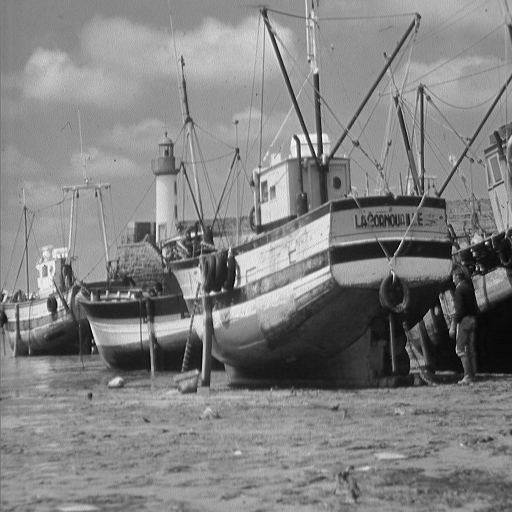
\includegraphics[scale=5] {boat}
	\caption{Obraz oryginalny boat.png}
\end{figure}

\begin{figure}[!htb]
	\centering
	\begin{minipage}[b]{0.4\textwidth}
		\includegraphics[scale=0.3]{boat_4x4_frame_compression_20_neurons.png}
		\caption{Obraz po kompresji używającej ramki (4x4) oraz 20 neuronów.}
	\end{minipage}
	\hfill
	\begin{minipage}[b]{0.4\textwidth}
		\includegraphics[scale=0.3]{boat_4x4_frame_compression_50_neurons.png}
		\caption{Obraz po kompresji używającej ramki (4x4) oraz 50 neuronów.}
	\end{minipage}
\end{figure}

\begin{figure}[!htb]
	\centering
	\includegraphics[scale=0.5] {lena}
	\caption{Obraz oryginalny lena.png}
\end{figure}

\begin{figure}[!htb]
	\centering
	\begin{minipage}[b]{0.4\textwidth}
		\includegraphics[scale=0.4]{lena_4x4_frame_compression_20_neurons.png}
		\caption{Obraz po kompresji używającej ramki (4x4) oraz 20 neuronów.}
	\end{minipage}
	\hfill
	\begin{minipage}[b]{0.4\textwidth}
		\includegraphics[scale=0.4]{lena_8x8_frame_compression_20_neurons.png}
		\caption{Obraz po kompresji używającej ramki (8x8) oraz 20 neuronów.}
	\end{minipage}
\end{figure}


\begin{figure}[!htb]
	\centering
	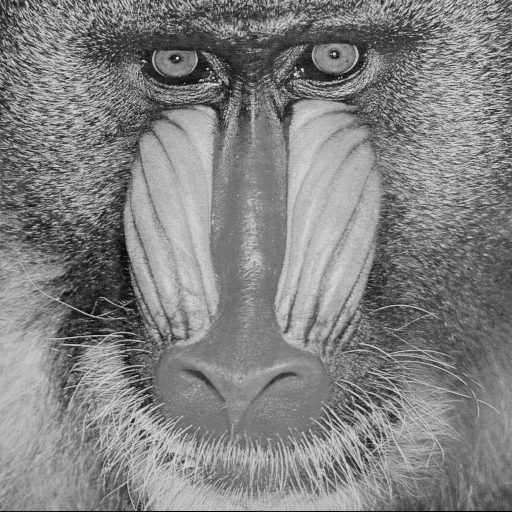
\includegraphics[scale=0.5] {mandrill}
	\caption{Obraz oryginalny mandrill.png}
\end{figure}

\begin{figure}[!htb]
	\centering
	\begin{minipage}[b]{0.4\textwidth}
		\includegraphics[scale=0.4]{mandrill_4x4_frame_compression_10_neurons.png}
		\caption{Obraz po kompresji używającej ramki (4x4) oraz 10 neuronów.}
	\end{minipage}
	\hfill
	\begin{minipage}[b]{0.4\textwidth}
		\includegraphics[scale=0.4]{mandrill_4x4_frame_compression_20_neurons.png}
		\caption{Obraz po kompresji używającej ramki (4x4) oraz 20 neuronów.}
	\end{minipage}
\end{figure}
	
		
}

\section{Dyskusja}
{Przy kompresji obrazu kluczowe jest dopasowanie wielkości ramki do samego rozmiaru obrazu. Jeżeli ramka jest zbyt duża w stosunku do obrazu wtedy wystąpią duże straty kompresji. Dla obrazów 512 x 512 ramka (4x4) jest bardzo dobrym rozwiązaniem, gdyż kompresja jest uzyskiwana w dość przyzwoitym czasie. Jednakże dla obrazu 256 x 256 taka ramka powoduje duże straty kompresji i zanik kształtów. Liczba 20 neuronów dla obrazów testowych wydaje się być sensownym rozwiązaniem, gdyż zapewnia wyniki w akceptowalnym czasie.}
\section{Wnioski}
{Kluczowym czynnikiem jest stosunek rozmiaru ramki oraz wielkości obrazu. Im mniejsza ramka tym większa szansa na wychwycenie szczegółów w obrazie. Ważnym aspektem jest również liczba neuronów, gdyż to ona decyduje ile grup powstanie dla barw w obrazie zdekodowanym.}

\end{document}
